%\section{Plenum Effect Study}

\section{Previous Work}

%Davis (Ref. 3) showed that with two adjacent $90^\circ$ holes, the flow coefficient at a choked condition can vary by as much as 6 percent depending on hole orientation. While Slater (Ref. 4) has developed a model for $90^\circ$ bleed holes based upon the Willis data, that model should be compared with single hole data where there is no interaction between adjacent holes.

A large library of flow coefficient data was developed beginning with McLafferty and Ranard \cite{McLafferty1958}, which was then expanded by Willis \cite{Willis1995}. The references built by these efforts cover a limited range of hole and geometries and bleed-hole orientations and are very configuration-specific. Syberg and Hickcox \cite{Syberg1973} also put some data together for 90 degree holes.

These experimental works paved the way for the normalization of bleed data by using a sonic flow coefficient.


% -----------------------------------------------------------
\section{Sonic Flow Coefficient}

Bleed configurations are characterized by the sonic flow coefficient ($Q_{\trm{sonic}}$), which is defined as

$$ Q_{\trm{sonic}} = \frac{\mdot_{\trm{bleed}}}{\mdot_{\trm{sonic}}} $$

%$$ \Qs = \frac{\mdot_{\trm{bleed}}}{\mdot_{trm{sonic}} $$

where $\mdot_{\trm{bleed}}$ is the mass flow rate through the bleed hole and $\mdot_{\trm{sonic}}$ is the ideal massflow rate under choked conditions assuming isentropic, sonic flow $(M=1)$ through the bleed hole. The $\mdot_{\trm{bleed}}$ is the flow rate given in the general form of

$$ \mdot_{\trm{bleed}} = \rho A v = p_t A M \cdot \qty(\frac{\gamma}{RT_t})^{\sfrac{1}{2}} \cdot \qty(1 + \frac{\gamma-1}{2}M^2)^{\sfrac{-\qty(\gamma+1)}{2\cdot\qty(\gamma-1)}} $$

and $\mdot_{\trm{sonic}}$ is in the form

%$$ \mdot_{\trm{sonic}} = p_t \Phi A_{\trm{region}} \qty(\frac{\gamma+1}{2}M^2)^{\sfrac{-\qty(\gamma+1)}{2\cdot\qty(\gamma-1)}} $$

\begin{equation} \mdot_{\trm{sonic}} = p_t \Phi A_{\trm{region}} \qty(\frac{\gamma}{RT_t})^{\sfrac{1}{2}} \qty(\frac{\gamma+1}{2})^{\sfrac{\minus\qty(\gamma+1)}{2\cdot\qty(\gamma-1)}} 
\label{eq:mdot_sonic}
\end{equation}

where $\Phi$ is the bleed hole porosity, $A_{\trm{bleed}}$ is the cross-sectional area of the bleed holes, $A_{\trm{region}}$ is the area of the total area of the region.

$$ \Phi = \frac{A_{\trm{region}}}{A_{\trm{bleed}}} $$


%$$ w_i^* = \frac{P_{t,e}\cdot A_b }{\sqrt{T_{t,e}}} \cdot \sqrt{\frac{\gamma\cdot g_c}{R_{air}}} \cdot \qty(\frac{\gamma+1}{2})^{\sfrac{-\qty(\gamma+1)}{2\cdot\qty(\gamma-1)}} $$

The ability of the bleed holes to extract bleed flow is represented by the sonic flow coefficient Qsonic. The bleed flow rate is calculated in the form of

$Q_{\trm{sonic}}$ thus represents the ability of the bleed hole to extract bleed flow. From experimental observation, %The bleed boundary condition requires $Q_{\trm{sonic}}$ to be evaluated. 
the values of $Q_{\trm{sonic}}$ varied for various Mach numbers with respect to the ration between the plenum static pressure and the total pressure of the inlet flow at the edge of the approaching boundary layer, $p_{\trm{plenum}}/p_{t\delta}$. The total pressure and total temperature at the edge of the boundary layer above the bleed region were used for the above equations.

At each Mach number, the $Q_{\trm{sonic}}$ varied with respect to the ratio between the plenum static pressure and the total pressure of the inlet flow at the edge of the approaching boundary layer, $p_{plenum}/p_{t\delta}$. The total pressure and total temperature at the edge of the boundary layer above the bleed region were used in \cref{eq:mdot_sonic}.

For each Mach number, the $Q_{\trm{sonic}}$, and so, the bleed flow $\mdot_{\trm{bleed}}$, increases as the plenum total pressure ratio is reduced. At some ratio, the bleed holes choke, and a maximum bleed rate is achieved. \cref{fig:willis_uncollapsed} illustrates the decrease in $Q_{\trm{sonic}}$ as the Mach number increases. This reflects the increased losses and increased difficulty in bleeding the flow as the Mach number increases.

\begin{figure}[htbp]
 \begin{center}
    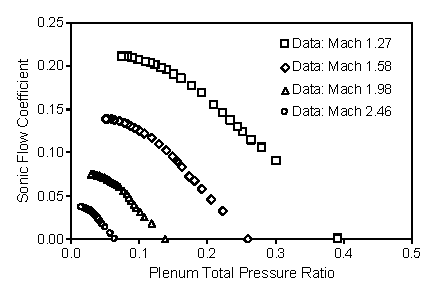
\includegraphics[width=3in]{willis_data_uncollapsed.eps}
     \caption{\LaTeX\ a very simple document from \cite{Slater2012}, who took it from \cite{Willis1995} Compile a very simple document.}
     \label{fig:willis_uncollapsed}
 \end{center}
\end{figure}


% -----------------------------------------------------------
\section{Mayer and Paynter}

Mayer and Paynter \cite{Mayer1994} created a model treats each bleed region like a porous wall extending from the front edge of the bleed band to the afte edge. The flow velocity normal to the wall is computed based on the local flow properties, the total bleed hole area, and a discharge coefficient function. The model yields the overall effects of bleed mass removal on the inlet flow but does not completely model local variations in bleed that undoubtely exist in either the streamwise or cross-stream direction. The model is based on the assumption that removing the correct amount of mass from the inlet as the normal shock moves forward over the simulated prous bleed region is much more important in an accurate simulation of the motion of the normal shock than how the mass flux removal is distributed over a bleed region.

The surface porosity is calculated $\Phi$, the wall velocity is computed, and the bleed hole sonic mass flow coefficient $Q_{sonic}$ is determined as a function of the bleed hole angle, the bleed plenum pressure, and the local flow proprties. $Q_{sonic}$ is interpolated from Syberg \cite{Syberg1973} and McLaugherty \cite{McLafferty1958}. pulled from a lookup table and bilinear interpolation is used to calculate the appropriate values of Qsonic.

The sonic flow coefficient is presented as a function of the ratio of bleed plenum pressure to freestream (boundary-layer edge) total pressure (Pplen/Pt,e). For the present study, the total temperature at the boundary-layer edge (Tt,e) is assumed to be the same as the total temperature in the wind tunnel plenum chamber (Tt,0).

The bleed hole sonic mass flow coefficient, Qsonic is determined as function of the bleed hole angle, the bleed plenum pressure, and the local flow proprties. 

$$ Q_{\trm{sonic}} = \frac{\dot{m}_{actual}}{\dot{m}_{max}} = f\qty(\alpha_{bleed},M_{local},\dfrac{P_{plenum}}{P_{Tlocal}}) $$

where $\dot{m}_{max}$ is the max theoretical flow at the local stagnation pressure and stagnation temperature. The local flow properties are taken at the wall for the inviscid flows or from the grid point that is just beyond the edge of the boundary layer for viscous flows. The q-sonic coefficient is a look-up table from the works of Syberg \cite{Syberg1973} and McLafferty \cite{McLafferty1958}.

Based on the definition for Qsonic and accounting for the surface pororisity $\Phi$, the effective bleed velocity magntitude is computed. The bleed flow is assumed to be normal to the flow domain boundary

The bleed model of Mayer and Paynter17 stands out as representing the current state of porous bleed modeling. This model was implemented within the Wind-US CFD code.23 The inlet analyses of Ref. 13 illustrated the use of this bleed model for a supersonic inlet analysis. The model allows the bleed rate to vary across the bleed region according to local conditions. This is important when shock waves are interacting with the bleed region. For example, behind the shock wave, the static pressures are greater, which should result in a greater amount of bleed flow than ahead of the shock. The local bleed rate is calculated by extracting flow properties from the flow field and using a table look-up of empirically-based sonic flow coefficients, Qsonic. The use of the Qsonic data for the bleed model requires the CFD code to compute the Mach number, total pressure, and total temperature at the edge of the boundary layer. However, it may be computationally complex and time-consuming to locate each grid point at the boundary layer edge. This has can be especially difficult for unstructured-grid CFD codes. Further, the edge of the boundary layer may not be well-defined, such as in the case of a shock / boundary layer interaction with extensive boundary layer separation. Thus, a different approach for using the Qsonic data is needed.

The bleed model as described has some drawbacks for CFD simulations. First, locating the edge of the boundary layer above a surface solution point in the bleed region may be a complex task for the CFD code. One approach is to estimate the boundary-layer thickness and determine the grid point at that distance from the surface. For structured grids one can indicate the number of grid points from the wall and follow a grid line from the boundary point out into the flowfield. For unstructured grids, a search algorithm would be needed because grid points may not follow a structured order away from the wall. A second concern is that the edge of the boundary layer may not be well-defined. Bleed is often desirable in regions of shock wave/boundary-layer interactions, but these flowfields may contain separated and distorted flows with a range of Mach numbers. Defining a boundary-layer edge may not be possible for such flowfields.

The porous bleed boundary condition is imposed for surface grid points located within the bleed region. The model assumes the region is continuously porous, and so, the flow through individual holes is not resolved nor are individual holes recognized.

This raised the question as to whether conditions at the surface near the bleed holes could be used to characterize the bleed data rather than referencing the data  to the conditions of the approaching boundary layer. Hence, a new scaling of the bleed data was developed that characterized the bleed data with respect to the surface conditions. The new scaling is presented here and is similar to that proposed by Davis \cite{Davis2012}; 

Slater and Davis proposed similar new scalings:

% -----------------------------------------------------------
\section{FIBE Effort}

A renewed effort at NASA Glenn led to some experimental work. 

from eichorn paper

The similarity of the normalization curves for the different Mach numbers has led the authors to seek a scaling that would collapses the curves to a single distribution. Initial efforts by Davis4 and Slater1 focused on the $90^\circ$ data of Willis et al. Both investigators took the approach of normalizing the bleed plenum pressure by the local surface static pressure, but Davis also included a coefficient to account for the slight overpressure of the bleed plenum at zero flow rates. For scaling the flow coefficient, the investigators took different approaches. Whereas Slater assumed for the $90^\circ$ hole case that the total pressure in the hole was approximately equal to the local surface static pressure, Davis established a purely empirical scaling based on the extrapolated choked value of the bleed plate. Slater’s correlation takes the form of:

% -----------------------------------------------------------
\subsection{Davis Model}

and Davis' scaled empirical correlation takes the form of:

% from eichorn paper

$$ Q_{scaled} = a + \dfrac{b}{1+\qty(\dfrac{P_{plen,scaled}}{c})^d} $$

\begin{table}[!htbp] \centering 
\begin{tabular}[c]{*{2}{|c}|} \hline
\textbf{Coefficient} & \textbf{Value}   \\ \hline
a   & -0.74177271 \\ \hline
b   &  1.7397157  \\ \hline
c   &  0.91473254 \\ \hline
d   &  3.2074431  \\ \hline
\end{tabular} 
\caption{Grid refinement in the plenum and patch sizing} 
\label{tab:davis1} \end{table}

where 

$$ P_{plen,scaled} - \frac{\dfrac{P_{plen}}{P_{t,e}}}{1.059\cdot\dfrac{P_w}{P_{t,e}}} = \dfrac{\qty(\dfrac{P_{plen}}{P_{t,e}})}{1.059 \cdot \qty(1+\dfrac{\gamma-1}{2}\cdot M^2_e)^{\sfrac{\minus\gamma}{\gamma-1}}} $$

$$ Q_{scaled} = \dfrac{Q}{e + f\cdot M_e^2 + g \cdot e^{M_e}} $$

\begin{table}[!htbp] \centering 
\begin{tabular}[c]{*{2}{|c}|} \hline
\textbf{Coefficient} & \textbf{Value}   \\ \hline
e   & -6.885241  \\ \hline
f   & -5.9569877 \\ \hline
g   &  5.9532869 \\ \hline
\end{tabular} 
\caption{Grid refinement in the plenum and patch sizing} 
\label{tab:davis2} \end{table}

Davis \cite{Davis2012} concluded that the scaling method presented by Slater (Ref. 4) was a better, but imperfect, fit for single-hole data than the scaling method Davis has previously proposed based upon a semi-empirical correlation of the data collected by Willis.


Slater \cite{Slater2009} developed a model for 90 degree bleed holes based on the Willis data for single-hole data where there is interaction between adjacent holes.


% -----------------------------------------------------------
\subsection{Slater Model}

The current work improves on the Mayer-Paynter bleed model by introducing a scaling of the Qsonic data for 90-degree bleed holes. The scaling is able to collapse the Qsonic data for various Mach numbers to a trend that can then be fitted with a quadratic polynomial which is only a function of the ratio of plenum static pressure to the surface static pressure. The scaling eliminates the requirement to compute the flow properties at the edge of the boundary layer. The curve fit also provides a rudimentary model for blowing within a bleed region, which can occur if there is recirculation within the bleed region in the presence of a shock. The next section discusses the bleed modeling and the scaling of the Qsonic data. The improved bleed model was implemented into the Wind-US CFD code



%The W is the flow rate given in the general form of $ W = \rho A v $

%The Wsonic is calculated by assuming isentropic conditions through the bleed holes with sonic flow (M = 1) within the bleed holes.

%in summary, 

%A quadratic curve was fitted to the scaled data of Fig. 2. The quadratic equation is


The new scaling is not based on a direct curve fit of the data and removes the Mach number at the edge of the boundary layer as a factor. The new scaling defined an alternative reference flow for the sonic flow coefficient of the form

$$ \mdot_{\trm{sonic}} = \Phi A_{\trm{region}} p_B \qty(\frac{\gamma}{RT_B})^{\sfrac{1}{2}} \qty(\frac{\gamma+1}{2})^{\sfrac{\minus\qty(\gamma+1)}{2\cdot\qty(\gamma-1)}}  $$

The total conditions were replaced with the static pressure and temperature at the boundary surface local to the bleed hole. The subscript $B$ denotes the surface or boundary value. The surface static pressure and temperature are both easily obtained in a CFD flowfield. 

The surface sonic flow coefficient was modified as

$$ Q_{\trm{sonic-B}} = \frac{\mdot_{\trm{bleed}}}{\mdot_{\trm{sonic-B}}} = \frac{\mdot_{\trm{bleed}}}{\mdot_{\trm{sonic}}} \qty(\frac{\mdot_{\trm{sonic}}}{\mdot_{\trm{sonic-B}}}) $$

The assumptions were made that the 

$$ \frac{p_{t\delta}}{p_B} = \qty(1+\frac{\gamma-1}{2}M_\delta^2)^{\sfrac{\gamma}{\qty(\gamma-1)}} $$

and 

$$ \qty(\frac{T_B}{T_{t\delta}})^{\sfrac{1}{2}} \approx 1 $$

The scaling was performed through the operations

$$ Q_{\trm{sonic-B}} = Q_{\trm{sonic}}\qty(\frac{p_{t\delta}}{p_B}) $$

and

$$ \frac{p_{\trm{plenum}}}{p_B} = \frac{p_{\trm{plenum}}}{p_{t\delta}}\qty(\frac{p_{t\delta}}{p_B}) $$

The effect of scaling the sonic flow coefficient data presented in \cref{fig:willis_uncollapsed} is shown in \cref{fig:willis_collapsed}. The scaled data collapsed along a trend such that the surface sonic flow coefficient only varied with respect to the static plenum pressure ratio $(p_{plenum}/p_B)$. The Mach number at the boundary-layer edge was removed as a factor.

\begin{figure}[htbp]
 \begin{center}
    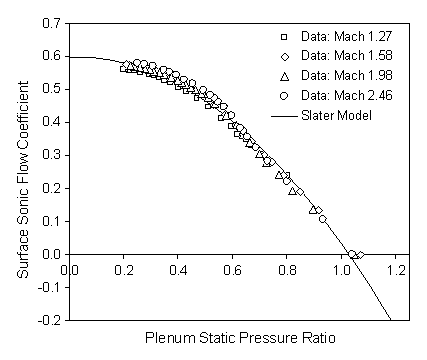
\includegraphics[width=3in]{willis_data_collapsed.eps}
     \caption{\LaTeX\ a very simple document from \cite{Slater2012}, who took it from \cite{Willis1995} Compile a very simple document.}
     \label{fig:willis_collapsed}
 \end{center}
 %\vspace{-0.2 in}
\end{figure}

The bleed flow for the improved bleed model is calculated as 

$$ \mdot_{\trm{bleed}} = Q_{\trm{sonic-B}} \cdot \mdot_{\trm{sonic-B}} $$

Both terms of the right-hand side of the above equation! are evaluated with respect to the plenum static pressure ratio. The plenum static pressure is either specified or computed based on other conditions such as those discussed in \cite{Slater2010} for a bleed plenum with a plenum exit with a fixed exit area.

A quadratic curve was fitted to the scaled data of \cref{fig:willis_collapsed}. The resulting quadratic equation was


$$ Q_{scaled} = \minus c \cdot \qty(P_{plen, scaled})^2 + b\cdot \qty(P_{plen, scaled}) + a$$

$$ Q_{\trm{scaled}} = \minus0.59799735P_{\trm{plen,scaled}}^2 + 0.03069346P_{\trm{plen,scaled}} + 0.59799735 $$

\begin{table}[!htbp] \centering 
\begin{tabular}[c]{*{2}{c}} \hline
\textbf{Coefficient} & \textbf{Value}   \\ \hline
a   & 0.59799735  \\ 
b   & 0.03069346  \\ 
c   & 0.59361420  \\ \hline
\end{tabular} 
\caption{Grid refinement in the plenum and patch sizing} 
\label{tab:slater} \end{table}

$$ P_{plen,scaled} = \dfrac{\qty(\dfrac{P_{plen}}{P_{t,e}})}{\qty(\dfrac{P_w}{P_{t,e}})} = \dfrac{\qty(\dfrac{P_{plen}}{P_{t,e}})}{\qty(1+\dfrac{\gamma-1}{2}\cdot M^2_e)^{\frac{\minus\gamma}{\gamma-1}}} $$

%$$ \dfrac{\qty(\dfrac{P_{plen}}{P_{t,e}})}{\qty(1+\dfrac{\gamma-1}{2}\cdot M^2_e)^{\dfrac{-\gamma}{\gamma-1}}} $$

$$ Q_{scaled} = \dfrac{Q}{\qty(\dfrac{P_w}{P_{t,e}})} = \dfrac{Q}{\qty(1+\dfrac{\gamma-1}{2}\cdot M^2_e)^{\frac{\minus\gamma}{\gamma-1}}} $$

The above equation is plotted along with the collapsed data in \cref{fig:willis_collapsed} and provides a good fit of the collapsed data. \cref{fig:willis_collapsed} indicates that at a static pressure ratio of approximately 1.03, the bleed flow is zero. The plenum pressure is slightly higher than the surface static pressure. This fact may indicate a dynamic or ram effect of the flow into the bleed holes, even at 90 deg. As the static pressure ratio approaches zero, the surface sonic flow coefficients approaches 0.6. This reflects the loss incurred in turning the flow into the bleed hole.

\cref{fig:syberg_data_collapsed,fig:mayer_data_collapsed} shows the application of the scaling to sonic flow coefficient data sets used in references 2 and 17. There is greater variation in the scaled values than shown in Fig. 2, but the curve fit of Eq. 13 does well in characterizing the data. The exception is the data for Mach 1.0 where the curve fit indicates lower values for the surface sonic flow coefficient. Note that the minimum Mach number of Fig. 1 upon which the curve fit was generated was Mach 1.27. The comparisons of Fig. 3 suggest that the curve fit may not work well for characterizing bleed rates below Mach 1.27. This is under continued study; however, given that most of the flow in supersonic inlets is above Mach 1.27, the curve fit should provide a good characterization of the bleed flow in supersonic inlets.

The scaling was applied to the sonic flow coefficients data sets used in \cite{Syberg1973,Mayer1994} to examine whether the scaling worked for other data sets. \cref{fig:syberg_data_collapsed} shows the results of that scaling along with the plot of Eq. (13). The data for Mach numbers of 1.3 and above seem to collapse together well; however, the variation is greated than observed for the data set of Willis et al. as shown in \cref{fig:willis_collapsed}. The curve fit of EQ. 13 represents both data sets for Mach numbers of 1.3 and above. However, the data for Mach 1.0 indicates higher values than indicated by the rest of the data and Eq. (13). This suggests that the scaling and Eq. (13) may have greater error in evaluating sonic flow coefficients at sonic and subsonic Mach numbers. However, the curve fit of Eq. (13) is accepted as a reasonable representation of the surface sonic flow coefficients for the time being, even at subsonic and sonic Mach numbers. Further modeling efforts should examine improving the curve fit for subsonic and sonic Mach numbers.

An additional benefit of the scaling of the sonic flow coefficient as expressed in Eq. 13 is that it provides a rudimentary model for blowing in a bleed hole. When the static pressure ratio is greater than 1.03, the value of the surface sonic flow coefficient is negative, which by Eq. 2 will result in a negative bleed flow or blowing. While large amounts of blowing are not intended in the design of a supersonic inlet, it is possible to experience recirculation within a bleed region. This can occur when a shock wave is interacting with the bleed region and the total bleed flow for the bleed region is small. The high pressures downstream of the shock cause pressurization of the bleed plenum, which forces the bleed plenum to blow flow out the bleed holes upstream of the shock where the local pressures are lower.



\begin{figure}[htbp] \begin{center}
    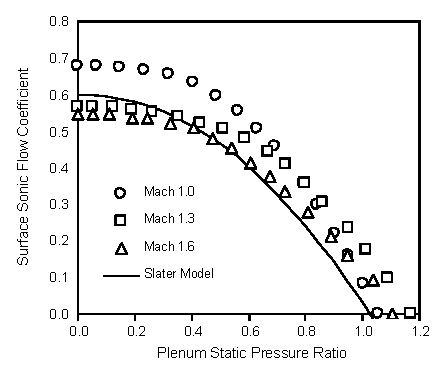
\includegraphics[width=3in]{syberg_hickcox_data_collapsed.eps}
    \caption{Syberg: \cite{Slater2012}, who took it from \cite{Willis1995} Compile a very simple document.}
     \label{fig:syberg_data_collapsed} \end{center}
\end{figure}

\begin{figure}[htbp]
 \begin{center}
    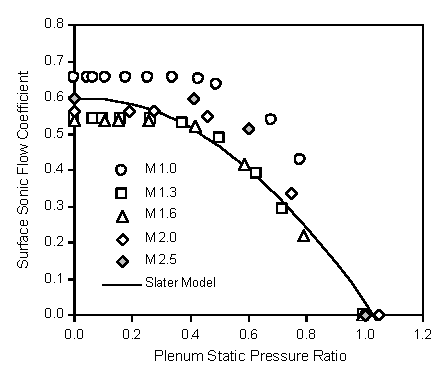
\includegraphics[width=3in]{mayer_paynter_data_collapsed.eps}
     \caption{\LaTeX\ a very simple document from \cite{Slater2012}, who took it from \cite{Willis1995} Compile a very simple document.}
     \label{fig:mayer_data_collapsed}
 \end{center}
\end{figure}

Data sets existed




% -----------------------------------------------------------
\subsection{Slater Model Modified}
% from slater journal paper

The original slater model yields a positive slope as $p_{plenum}/p_B < 0.02585 $, contradicting the expectation that the sonic flow coefficient continually increases as the static plenum pressure approaches zero.

by Andrew Dorgan of the Boeing Company, private communications, Apr. 2011

$$ Q_{sonic-B} = -0.57 \cdot \qty(\frac{p_{plenum}}{p_B})^2 $$

This alternative curve-fit differs in shape only slightly and not distinguishable if plotted.

%These models provide a rudimentary model for blowing in a bleed hole.





% -----------------------------------------------------------
%\section{Slater Model}
% note


% -----------------------------------------------------------
\subsection{Results from Phase I}
% note
strenghts and weaknesses of slater model. can include plot from eichorn paper

Both methods collapse the $90^\circ$ data fairly well. The plot shows Elater's correlation fits the present data better which isn't unexpected since Davis' correlation was based on an empirical fit of the extrapolated choke points of the multi-hole data. Slater's correlation seems to fit the lower Mach number data better with increasing deviation as the Mach number is increased. However, even the lowest Mach number data deviation from the Slater correlation near the choke point, implying that n adjustment for the number of bleed hole rows, and potentially the hole spacing, may be required.

The above wall static pressure scaling (slater) assumes that the total pressure in the hole is nearly the same as the surface wall static pressure. This is likely a reasonable assumption for holes with large inclination angles as all the freestream total pressure is lost turning the flow through a large angle. As the inclination angle is reduced, however, some of the freestream total pressure is expected to be recovered in the hole and it is thus expected that the above scaling will not work as well, particularly at high flow rates. This suggests that a physics-based model must account for the total pressure recovery in the hole which may be a function of a number of parameters.

% -----------------------------------------------------------
\subsection{Results from Phase II}
Davis \cite{Davis2012} and Eichorn \cite{Eichorn2013} present Phases I and II, respectively, of a Fundamental Inlet Bleed Experiments study at NASA Glenn Research Center.

Several examples of collapsed data using the equations above for specific bleed holes are given in Figure 7. Unlike the data collected by Davis (Ref. 6), the data from many of these plates collapse very well when this scaling is applied. Of particular note are plates with the smallest nominal thickness-todiameter ratio (t/D=0.25), Figure 7(a) to (c) (top row of plots), which collapse very well independent of hole angle. That these plates collapse well isn’t necessarily surprising inasmuch as very thin plates do not have the same internal shock structure as thicker plates do. Figure 7(d) to (f) (middle row of plots) display the collapse for hole configurations where the nominal thickness-to-diameter ratio is 2.0 and the hole angle is $55^\circ$ and in this case the collapse appears to have higher degree of scatter, however there is little apparent trend in Mach number. The final selection, Figure 7(g) to (i), present the $20^\circ$ hole data and as Davis (Ref. 6) concluded, the scaling does not work particularly well for $20^\circ$ holes. These have a distinct difference in magnitude where the maximum scaled sonic flow coefficient increases with Mach number. Further this tendency is related to the hole diameter as the smaller hole diameters show less separation between the curves.

A comparison of all collapsed data is shown in Figure 8. The values for the $20^\circ$ holes are noticeably larger than those of the $90^\circ$ and $55^\circ$ holes which themselves form two distinct groups. The $90^\circ$ holes seem to form tight bands for specific thickness-to-diameter ratios, however both the $55^\circ$ and $90^\circ$ holes only show a loose grouping where that ratio is small.


% notes
from slater conf paper

The methods of computational fluid dynamics (CFD) have been applied to the aerodynamic analysis of supersonic inlet flows containing bleed regions.11-13 The small scale of the bleed holes has resulted in the typical approach of modeling the effects of porous bleed through the use of surface boundary conditions. Various bleed boundary condition models have been reported by a number of researchers.14-22 These models follow the general approach of assuming the bleed region to be a continuously porous surface. The solution points located within the bleed region are computed as boundary conditions in which the local bleed rates and velocity components are computed. The individual bleed holes are not identified nor are the details of the flow within the bleed holes computed. The models attempt to capture the collective behavior of the bleed holes.



% -----------------------------------------------------------
\section{Experiment}
% from Slater conf paper

The experiment \verb|cite willis davis hingst| that was used for validation was performed in the NASA Glenn Research Center 1 ft by 1 ft Supersonic Wind Tunnel (SWT) measuring mass flow rate through bleed holes at various Mach numbers. The quantities that were used in the validation were the boundary layer thickness and momentum thickness of the naturally boundary layer along the wind tunnel wall, the bleed hole diameter, the bleed hole depth, and the pressure ratios used in the experiment to draw air through the bleed hole. A plenum sat below the hole where the plenum pressure could be varied (which controlled the pressure ratio through the hole), varying the massflow rate through the hole.

D = 0.236 in.
L = 2D

\begin{table}[!htbp] \centering 
\begin{tabular}[c]{*{2}{l}} \hline
\textbf{Parameter} & \textbf{Value}   \\ \hline
Mach Number   & 2.46  \\ 
Total Pressure [psia]   & 25.0 \\ 
Reynolds Number per foot   &  5.15E+06 \\ 
Boundary Layer Thickness [in.] & 0.5079 \\ \hline
\end{tabular} 
\caption{Grid refinement in the plenum and patch sizing} 
\label{tab:bl} \end{table}

\begin{table}[!htbp] \centering 
\begin{tabular}[c]{*{5}{c}} \hline
\textbf{Parameter} & \textbf{Value} & \textbf{Grid Size} & \boldmath{$Q_{sonic}$} & \boldmath{$\Delta Q_{sonic}$}    \\ \hline
SA & 0.08 & Small & 0.0273 & 5.52\% \\ \hline
\end{tabular} 
\caption{Grid refinement in the plenum and patch sizing} 
\label{tab:grid_convergence} \end{table}

\begin{table}[!htbp] \centering 
\begin{tabular}[c]{*{2}{c}} \hline
\textbf{Parameter} & \textbf{Value}  \\ \hline
D & 0.236 \\
L & 2D \\
Ref & 2.46 \\
Mach & 2.46 \\
Re & 5.15E+06 / ft \\
$P_t$ & 25.0 psia \\ 
$\delta$ & 0.5079 in. \\ \hline
\end{tabular} 
\caption{Grid refinement in the plenum and patch sizing} 
\label{tab:stats} \end{table}

The CFD simulations involved a single 90-degree bleed hole with a diameter D = 0.236 inches and length of L = 2 D. The hole was located in a disk mounted flush with the bottom of the test section of the 15cm x 15cm wind tunnel at the NASA Glenn Research Center. The boundary layer over the plate was the naturally-occurring boundary layer on the bottom surface of the wind tunnel. The flow conditions and boundary layer profile approaching the bleed region were measured with a translating pitot probe and wall static pressure ports. The reference station for the approach flow was located 2.46 inches ahead of the center of the bleed hole. The bleed plenum was attached to the outside of the wind tunnel with ducting to a vacuum exhaust. The plenum was cylindrical with an inside diameter of 2.874 inches and an axial length of 3.50 inches. The axis of the plenum was parallel to the axis of the bleed hole. A vacuum chamber was used to establish the bleed flow rate, which was measured using a calibrated nozzle. The uncertainty of the experimental data was reported as $\pm1.5 \%$ for total pressures, and $\pm 1 \%$ percent for values of Qsonic. 

%The CFD simulations were performed at a Mach number of 2.46. Geometric and flow symmetry was assumed and allowed only half of the tunnel, bleed hole, and plenum to be simulated. A reflection boundary condition was used on the symmetry plane. The bottom and side of the tunnel were specified with adiabatic, no-slip boundary conditions. The top of the tunnel was specified as an inviscid wall so as to require less grid points to resolve the boundary layer, which was assumed not to influence the flow through the bleed hole. 

The inflow boundary was positioned an axial distance of 38.46 inches ahead of the center axis of the hole. This position was determined to provide a turbulent boundary layer at the reference location that matched the reference boundary layer profile and edge conditions of the experiment. 

The  conditions at the edge of the boundary layer were a Mach number of 2.46, total pressure of 25.0 psia, and a Reynolds number of 5.15E+06 / ft. The boundary layer thickness was 0.5079 inches. 

The outflow boundary was positioned 5.0 inches downstream of the center axis of the bleed hole and a first-order extrapolation boundary condition was used for the supersonic outflow. The plenum was modeled as a cylinder with a converging-diverging nozzle directed downward for the outflow for the plenum. The exit for the plenum nozzle was located 6.472 inches below the bottom wall of the tunnel and a subsonic outflow boundary condition was imposed in which the static pressure was specified. The bleed flow reached very low speeds within the plenum and the intent of the nozzle was to create a smooth exit for the bleed flow from the plenum. The walls of the plenum and bleed hole were specified as adiabatic, no-slip boundary conditions.

Initial solutions for the tunnel boundary layer indicated that a wall spacing of 2.4E-04 inches provided a non-dimensional wall spacing of y+  1.0. The grid distribution was determined using a hyperbolic-tangent method with end-spacings specified. The number of grid points along an edge was selected such that the maximum grid stretching was less than $15\%$. Within the bleed hole, the maximum spacing was limited to 0.005 inches (0.02 D), which set the level of maximum resolution of the flow within the bleed hole. This grid established the highest resolution of the flow field for the grid convergence study (fine grid). The resulting grid contained 678375 grid points within the bleed hole. The entire grid contained over 6.66 million grid points with over half of the grid points located within 3 diameters of the bleed hole and within the plenum. 

The CFD flow solution was initialized with Mach 2.46 flow within the tunnel and very low speed (Mach 0.01) flow within the bleed hole and plenum with a static pressure equal to the tunnel static pressure. An inviscid boundary condition was imposed at the plenum nozzle exit so as to initially not allow any bleed flow. This created the zero-bleed solution. Flows with bleed were then simulated by imposing the subsonic outflow boundary condition at the plenum nozzle outflow and specifying reduced values of static pressure to draw out the plenum flow. Subsequently lower values of exit static pressure yielded a sequence of solutions with greater bleed flow until the maximum bleed flow was obtained with essentially a vacuum within the plenum. 

At each solution point, the iterative convergence was examined by monitoring the amount of bleed flow and the plenum static pressure. The bleed flow was measured within the plenum nozzle where the flow was entirely directed toward the exit without recirculation, which ensured an accurate evaluation of the mass flow. The plenum pressure was obtained by mass-averaging the static pressure on a horizontal plane near the start of the nozzle. 

The grid convergence was examined by solving the flow field on three grids of subsequent coarseness. The Wind-US code allows grid sequencing in which allows the solution to be computed on coarser grids obtained by skipping a number of grid points. This allowed the grid sensitivity study to be conducted without having to generate coarser grids. The medium grid was obtained by skipping every other grid point. The coarse grid was obtained by skipping three grid points. This can also be used to accelerate convergence by starting the initial solution on the coarse grid. Table 2 lists the results on the coarse (0.08D), medium (0.04D), and fine (0.02D) grids for both the Spalart-Allmaras (S-A) and Menter SST turbulence models. The simulations were performed with the bleed rate approximately $75\%$ of its maximum value. As can be seen, the bleed rates showed little variation between the medium and fine grids. This can also be seen in Fig. 8 with the plot of the data of Table 2. The value of Qsonic from the experiment is also plotted in Fig. 8. 

The simulations with the S-A and SST turbulence models are essentially the same with both indicating Qsonic values approximately $25\%$ higher than the experimental data. However, it was discovered that the approach Mach number for these simulations was only 2.38 rather than 2.46. The inflow conditions were subsequently changed to obtain the correct inflow Mach number of 2.46 for the remaining simulations. However, this did not change the conclusion that further simulations could be conducted using the medium grid with a resolution of 0.04 D using the Menter SST turbulence model. Figure 8 shows the result of simulation D which was conducted on the medium grid with the Menter SST turbulence model.

The flow conditions 

talk qualitatively about the physics in the hole

some issues that i faced was that the flow was very unsteady, probably due to a timestep issue. talk a lot about this

\begin{figure}[htbp] \begin{center}
    \includegraphics[width=3in]{slater_cfd_plot.eps}
    \caption{Syberg: \cite{Slater2012}, who took it from \cite{Willis1995} Compile a very simple document.}
     \label{fig:asdf} \end{center}
\end{figure}

\begin{table}[!htbp] \centering 
\begin{tabular}[c]{*{5}{c}} \hline
& \textbf{Small Patch} & \textbf{Medium Patch} & \textbf{Large Patch} & \textbf{Complete Suction} \\ \hline
\textbf{Coarse Grid} & 14.8\% & 3.4\% & 11.1\% & 2.0\% \\
\textbf{Medium Grid} & 12.3\% & 4.6\% &  3.0\% & 1.8\% \\
\textbf{Fine Grid}   &  9.7\% & 2.2\% &  0.0\% & 1.5\% \\ \hline
\end{tabular} 
\caption{Grid refinement in the plenum and patch sizing} 
\label{tab:results} \end{table}

%\figSmallPatch

% ======================================================= Grid Independence
%\subsection{Grid Independence}

%\begin{figure}[tbp!] \centering
%	\begin{subfigure}{0.5\textwidth}
%		\centering
%		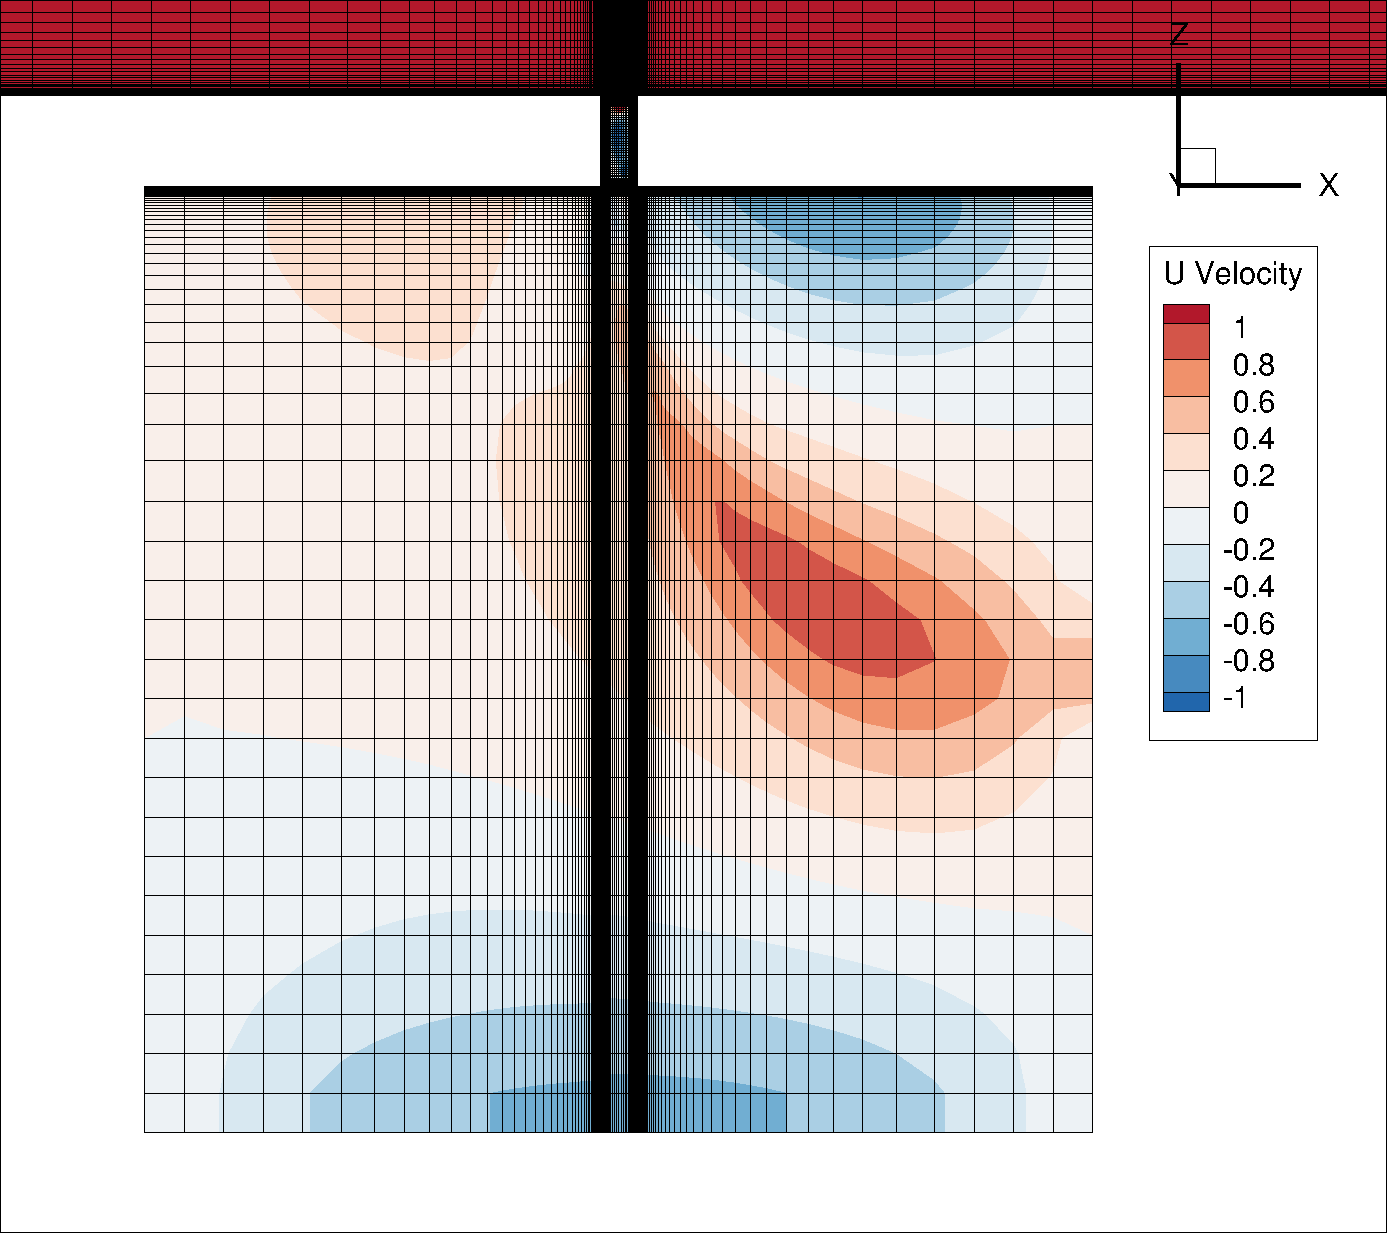
\includegraphics[width=0.5\linewidth]{1-1_grid.png}
%		\caption{1} \end{subfigure}%
%	\begin{subfigure}{0.5\textwidth} 
%		\centering
%		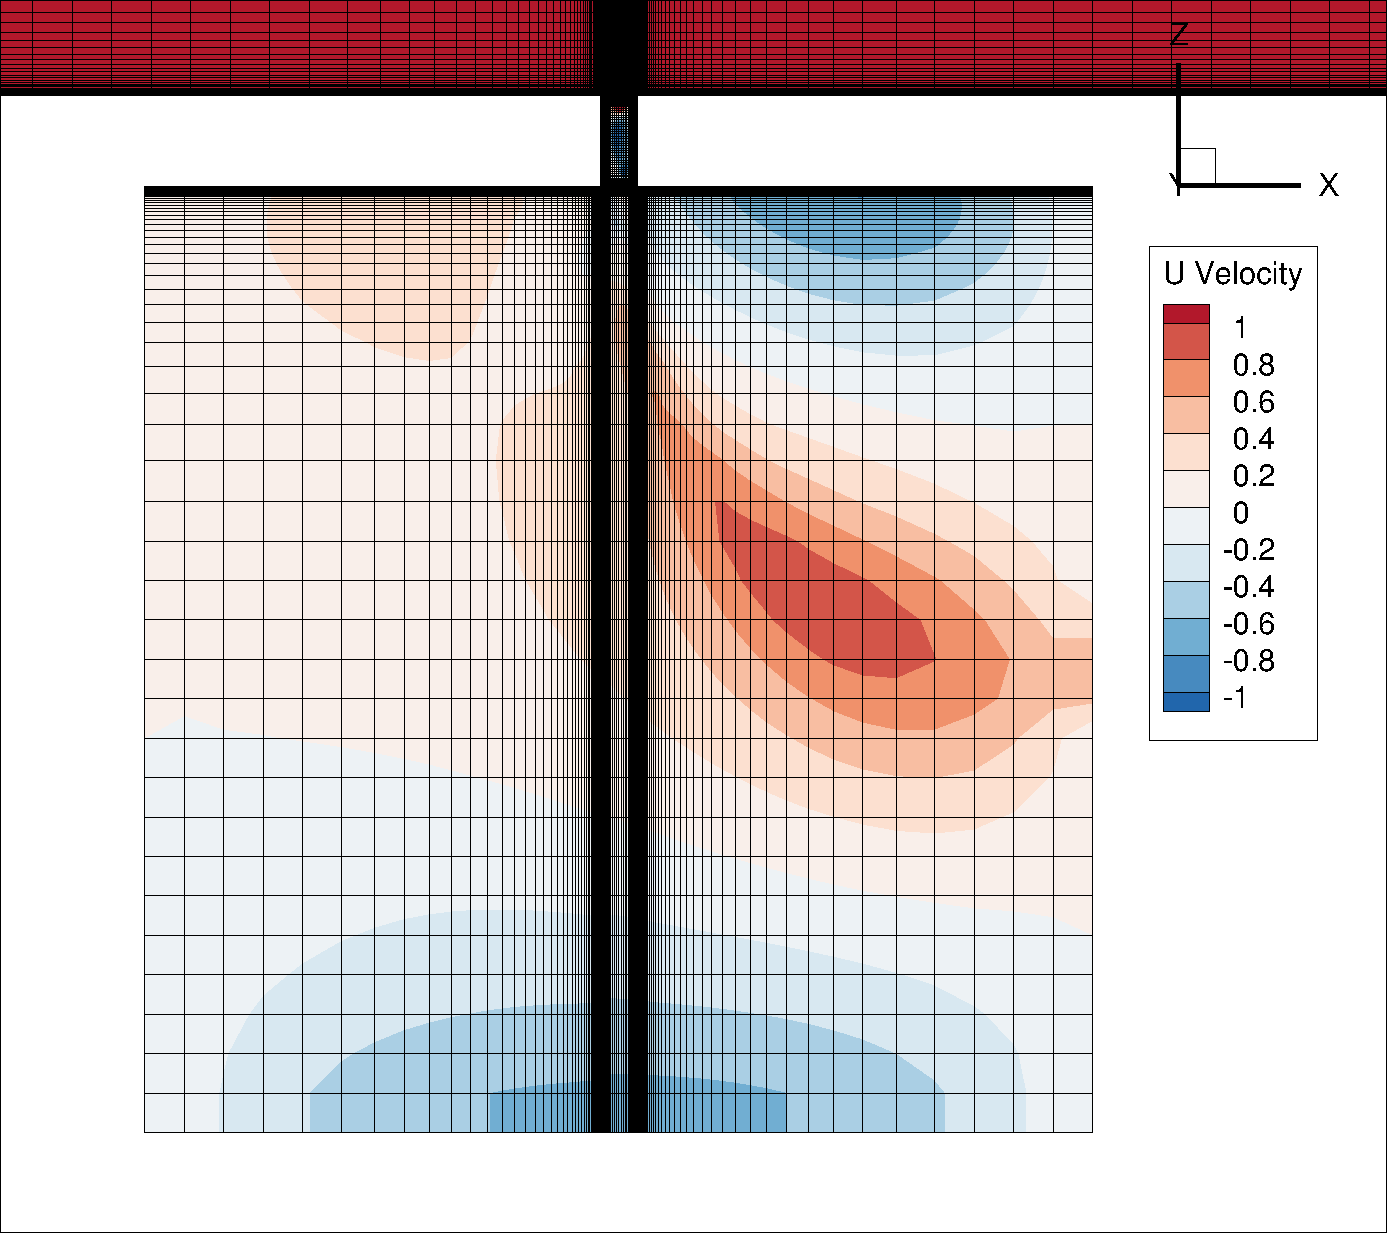
\includegraphics[width=0.5\linewidth]{1-1_grid.png}
%		\caption{1} \end{subfigure}
%\caption{hihi}
%\label{fig:small}
%\end{figure}

% \begin{figure}[tbp] \centering
% \begin{subfigure}{.32\textwidth} \centering
%   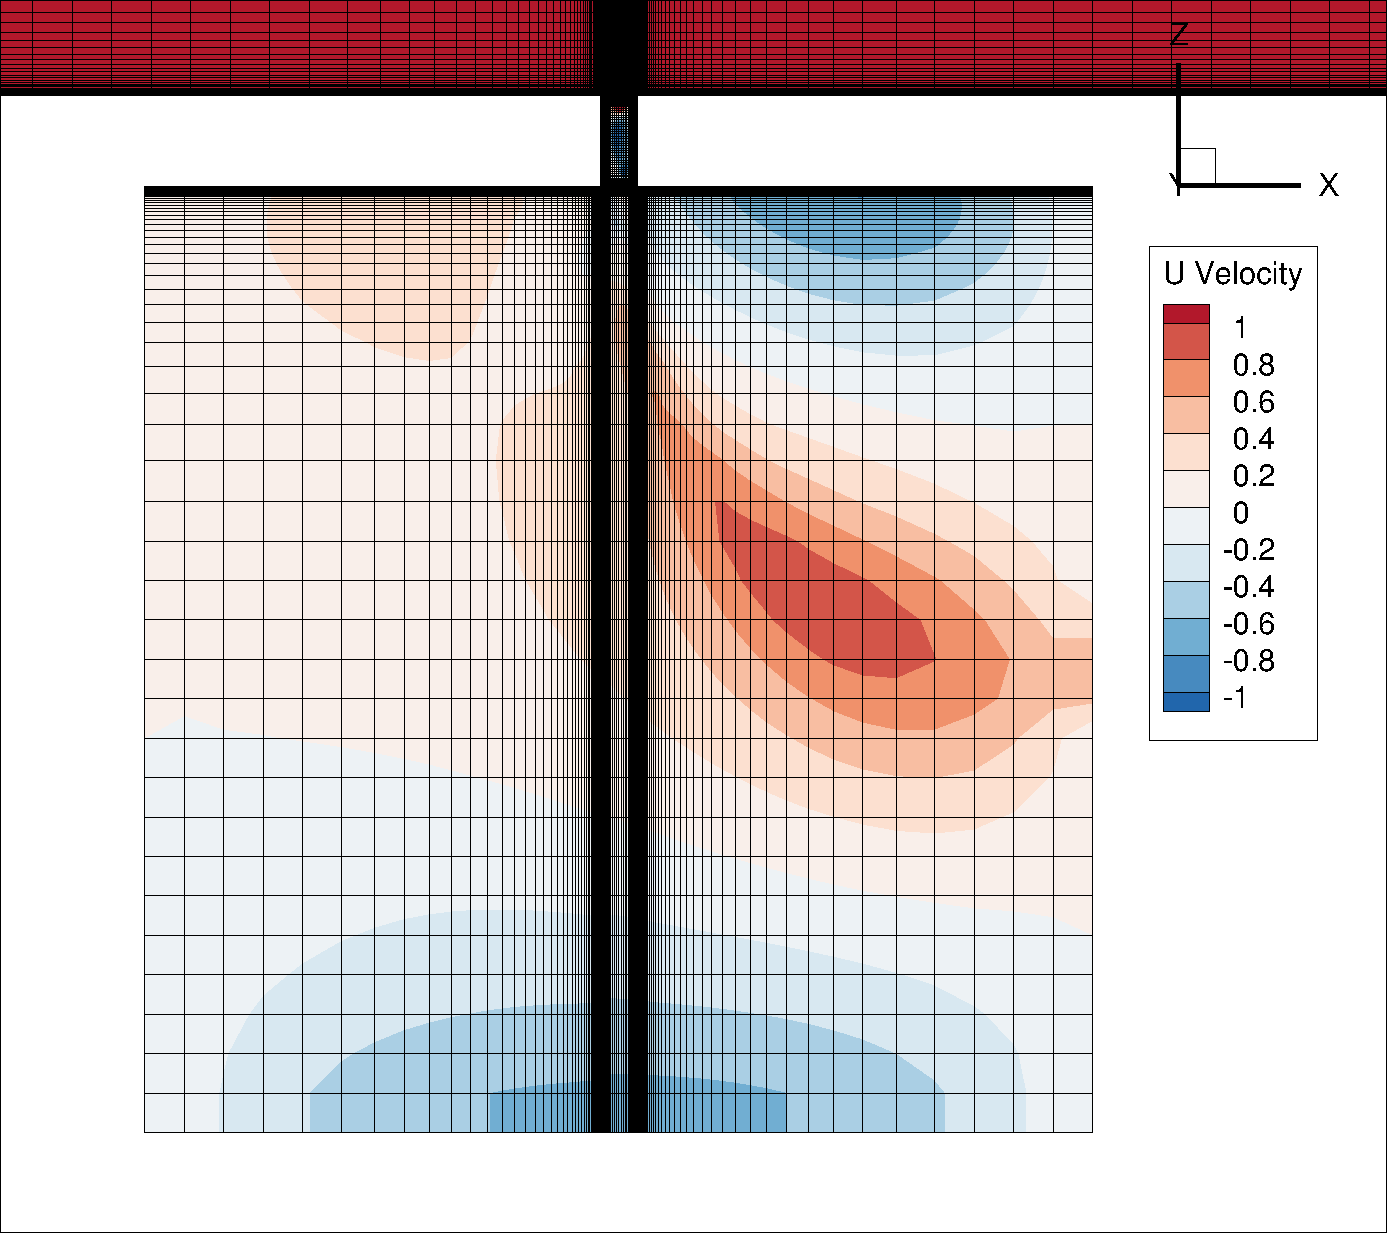
\includegraphics[width=1\linewidth]{1-1_grid.png}
% \end{subfigure}%
% \begin{subfigure}{.32\textwidth} \centering
%   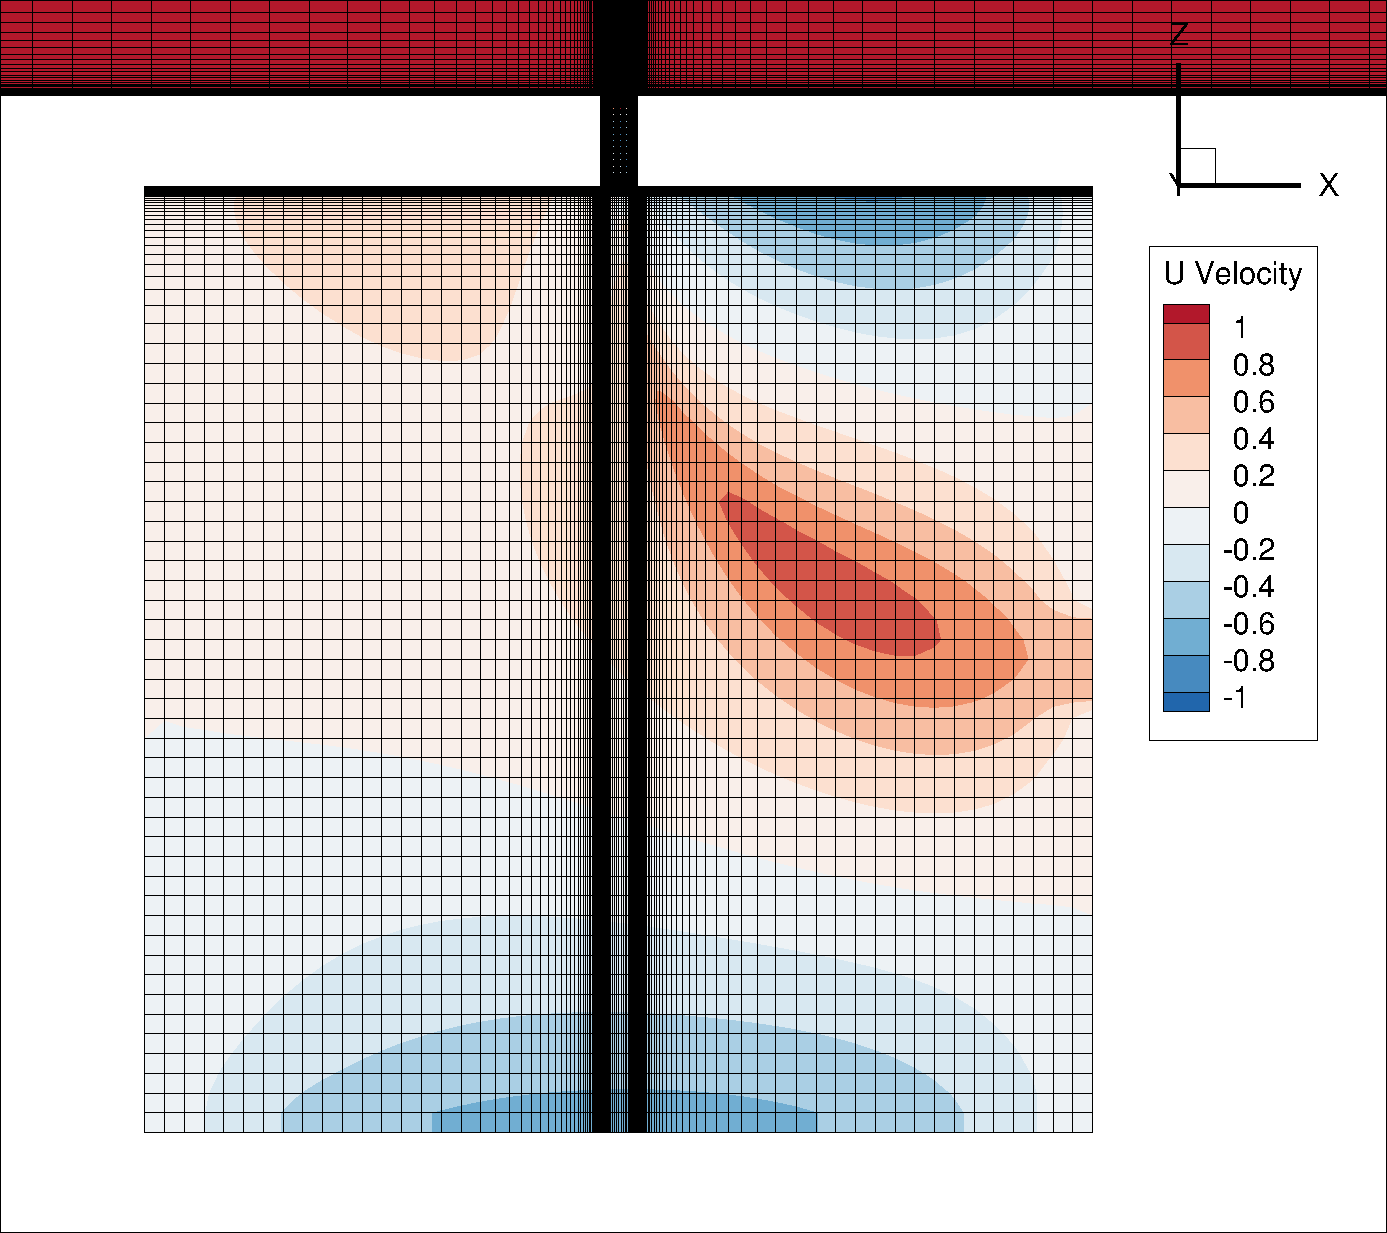
\includegraphics[width=1\linewidth]{1-2_grid.png}
% \end{subfigure}%
% \begin{subfigure}{.32\textwidth} \centering
%   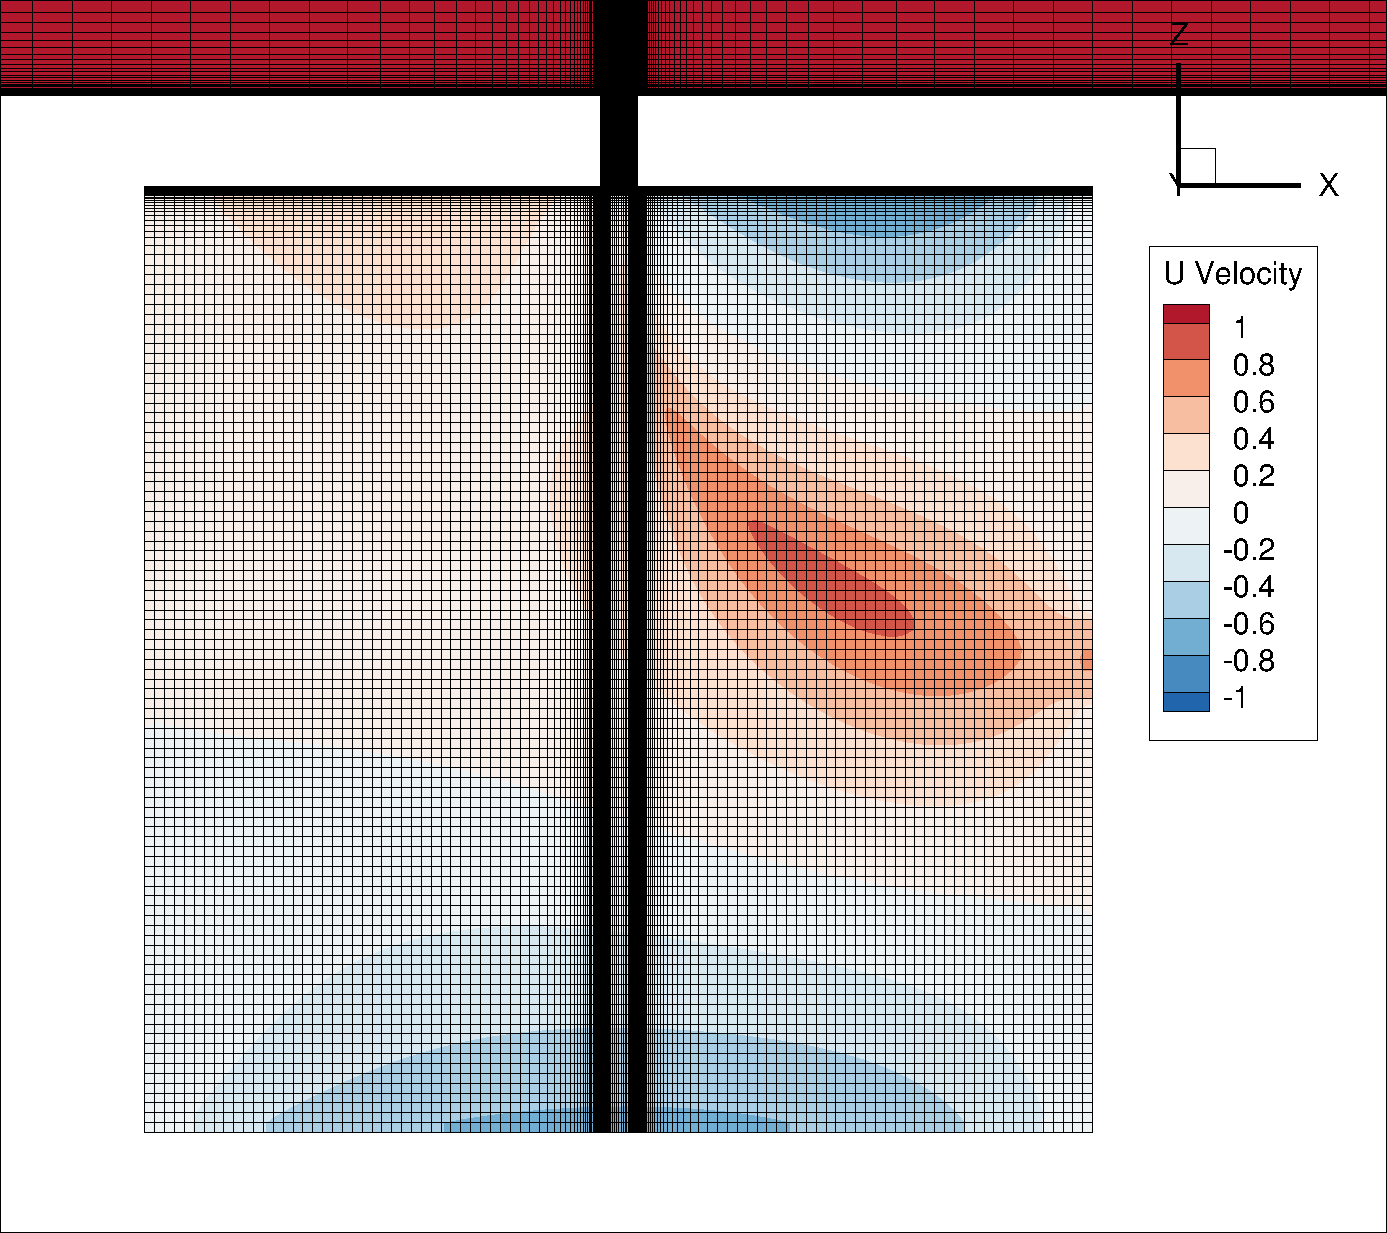
\includegraphics[width=1\linewidth]{1-3_grid.png}
% \end{subfigure}
% \begin{subfigure}{.32\textwidth} \centering
%   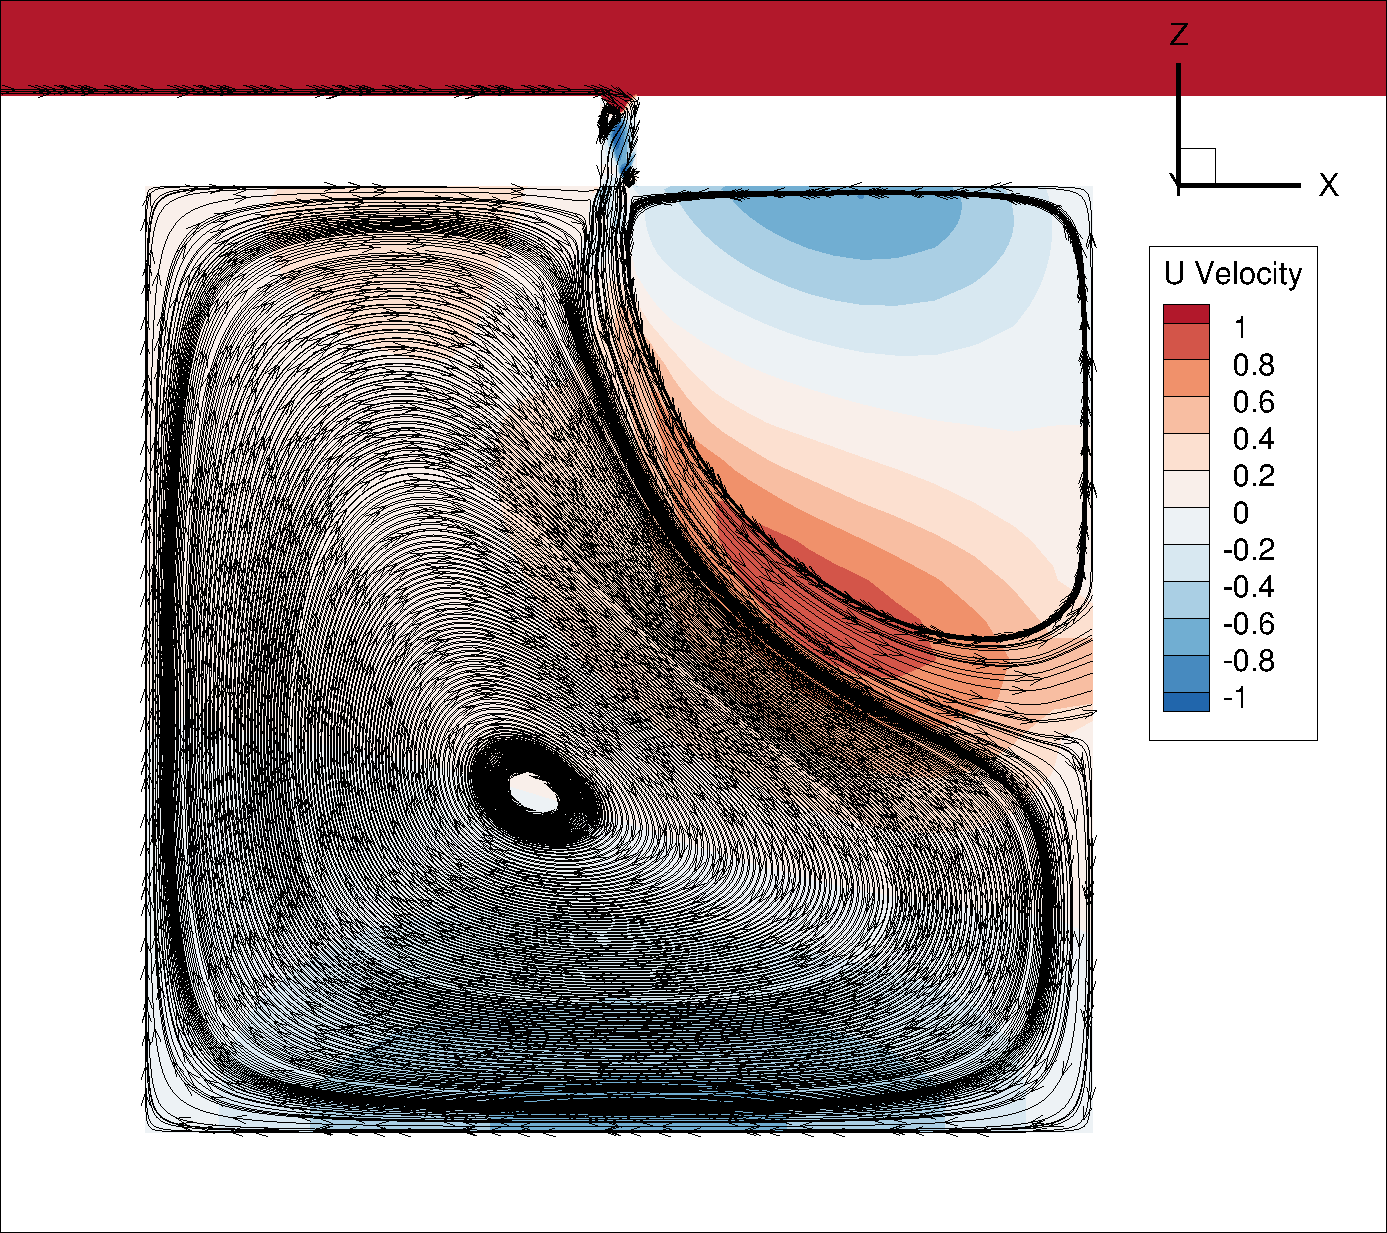
\includegraphics[width=1\linewidth]{1-1_streamlines.png}
% \end{subfigure}%
% \begin{subfigure}{.32\textwidth} \centering
%   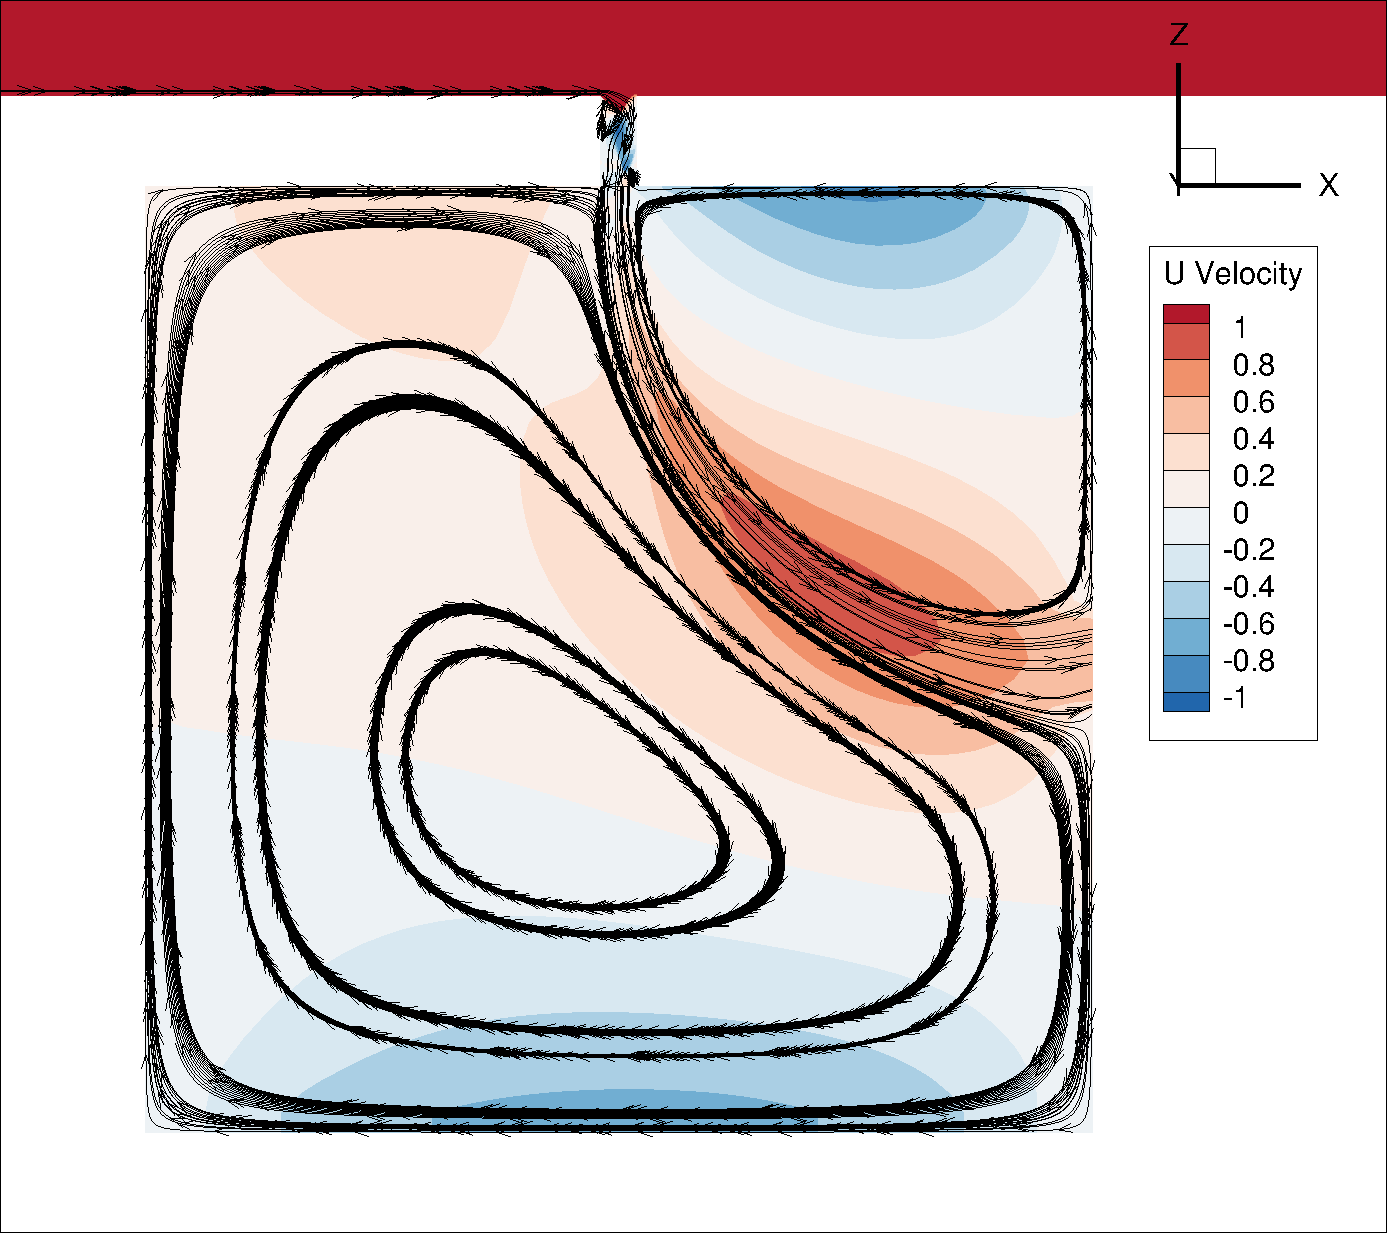
\includegraphics[width=1\linewidth]{1-2_streamlines.png}
% \end{subfigure}%
% \begin{subfigure}{.32\textwidth} \centering
%   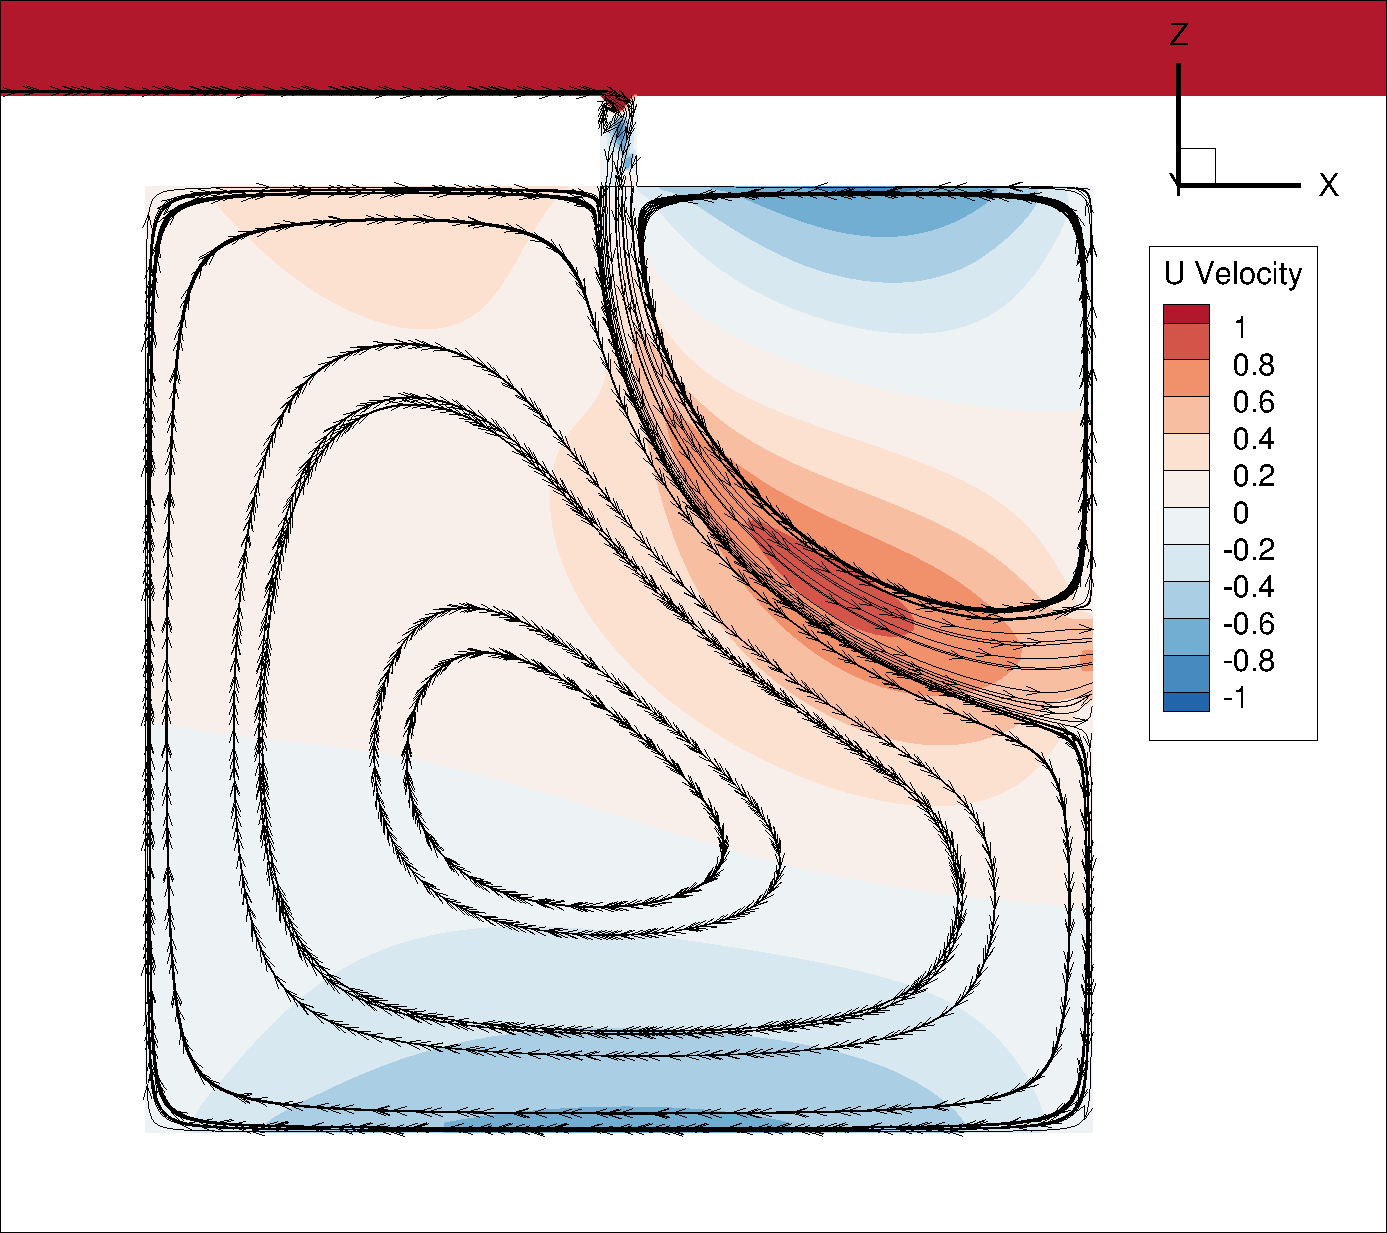
\includegraphics[width=1\linewidth]{1-3_streamlines.png}
% \end{subfigure}
%   \caption{Grid resolution study of the contours of u-velocity and streamlines for % the small patch}
%   \label{fig:small}
% \end{figure}

% ======================================================= Time Independence
%\subsection{Time Independence}

% ======================================================= Results
%\subsection{Results}